\documentclass{standalone}
\begin{document}
	\subsection*{Lung Extraction}
	
	This preliminary step is performed before both training and labeling and involves the managing of the HU, the isolation of lung regions and the removal of the main bronchial structures.
	
	The registration of the HU on a common space is necessary to overcome the issues that may raise from the different padding values and multiplicative constant for HU computation (equation\,\ref{eq:HU}) used by the different manufacturer of the CT scans. The $k$ constant in the HU definition (equation\,\ref{eq:HU}) may change according to the scan manufacturer or scan model. During the scan acquisition, all the regions outside the CT tube aren't sampled, so to obtain a square $N\times N$ image for each slice some padding values are added, which different values according to the scan manufacturer. This registration allows to overcome some issues that may raise during the conversion of the image from $16$ to $8$ bit unsigned integers, required to operates with \textsc{OpenCV} functions.
	
	
	Lung segmentation is a pivotal pre-processing step in many image analysis such as identification and classification of lung pathologies~\cite{ART:Johannes}. The lung isolation allow us to fund a mask for the lung regions, and thus excluding  all the body regions, the CT tube and the extra-lung organs like intestine and heart, avoiding the formation of false positives.
	
	Automatic lung segmentation algorithm are typically developed and tested on limited datasets and usually over a limited spectrum of visual variability by containing mainly cases without severe pathologies~\cite{ART:Johannes}. Rule based approach, like thresholding, region growing, ect, usually fails for CT sans of patients with severe Interstitial Lung Disease (ILD), as we can see in \figurename\,\ref{fig:UNetVSThr}. To achieve the lung segmentation I've used a pre-trained U-Net~\cite{ART:Johannes}~\cite{REP:lungmask}. 
	\begin{figure}[h!]
		\centering
		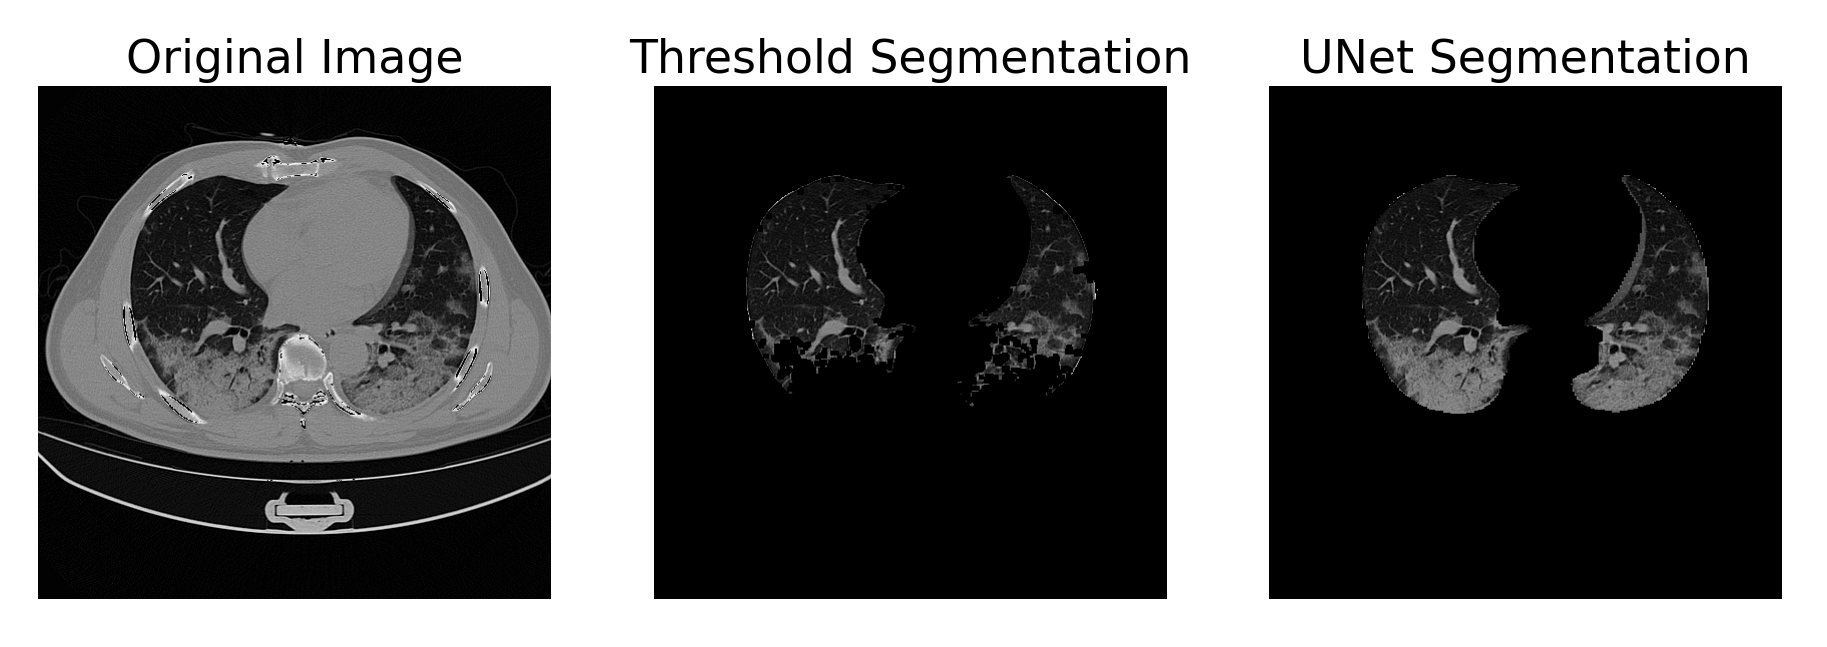
\includegraphics[scale=.5]{UNetVSThr.png}
		\caption{From left to right the original CT scan of a patient with severe ILD, the lung segmented by threshold and it's connected components, and lung segmentation achieved by the pre-trained U-Net. We can clearly see the missing areas in the first segmentation, correctly identified in the U-Net one.}\label{fig:UNetVSThr}
	\end{figure}

	This kind of segmentation includes in the lung region also motion artifacts and bronchial structures, which we will see are the principal causes of false positives. To achieve a better segmentation a refinement process is performed, which aims to remove the main bronchial structures form the selected lung regions. 

	Bronchi have an elongated shape respect to the other structure which usually are rounded: the basic idea was to use this kind of information. In order to perform this task, I have  computed the covariant matrix of the derivative in a neighborhood (\ref{eq:CovMat}) and the corresponding eigenvalues. 
	\begin{equation}\label{eq:CovMat}
		M = \begin{bmatrix} \sum _{S(p)}(dI/dx)^2 & \sum _{S(p)}dI/dx dI/dy \\ \sum _{S(p)}dI/dx dI/dy & \sum _{S(p)}(dI/dy)^2 \end{bmatrix}
	\end{equation}
	
	If a particular regions has an elongated shape, one of the eigenvalues (corresponding to the eigenvector in the direction of the structure) will be higher than the other, otherwise both eigenvalues have are lower. I have applied this filter on each slice of the scans and took a map of the maximum eigenvalues. 
	\begin{figure}[h!]
		\centering
			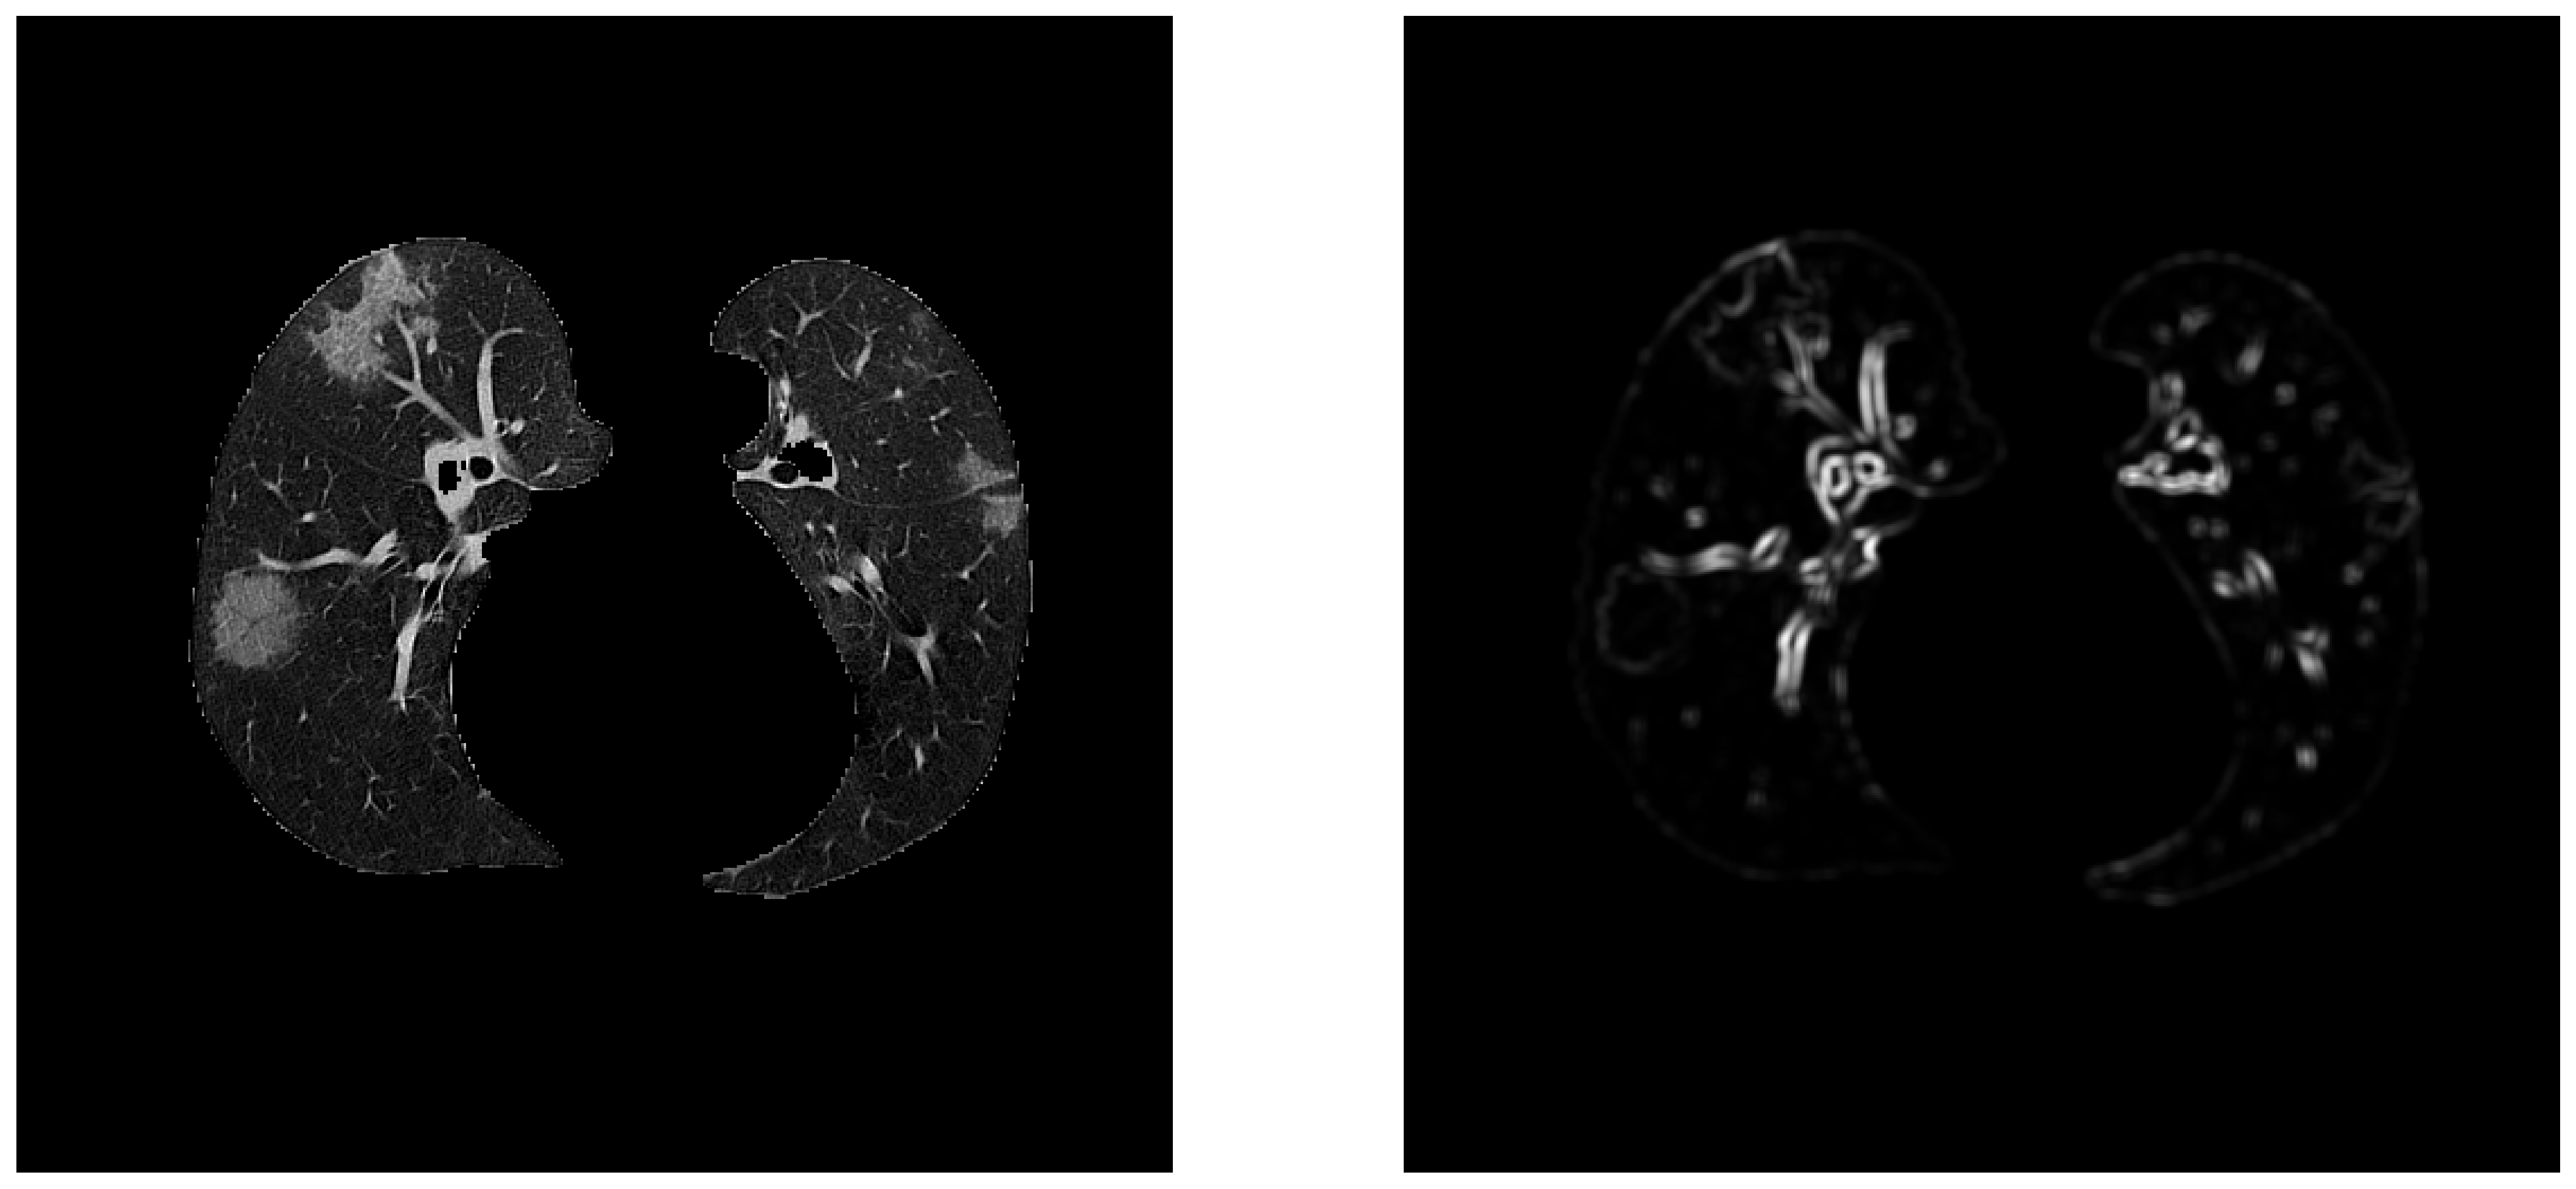
\includegraphics[scale=.3]{MaxEigenVal.png}
		\caption{From left to right: lung regions selected by the U-Net; ,maximum eigenvalues map of the lung. As we can see the U-Net does not exclude the bronchial structure from the lung, on the other hand, the maximum eigenvalues map delineates very well these regions. I have used this map to remove the unwanted bronchial regions.}\label{fig:MaxEigenval}
	\end{figure}

	In \figurename\,\ref{fig:MaxEigenval}, I've displayed the image after the lung segmentation by the neural network, and the corresponding eigenvalues map. As we can see the higher values of the map corresponds to the edges of the main bronchial structures. To create the mask for these structures I have applied a fixed threshold to map. Since the main bronchial structures are large, this process is able to remove only part of the edges, but the inner structure is preserved. In order to refine the segmentation, this process is repeated a second time, allowing a more accurate exclusion of the structures.
\end{document}